%%% Illustration of the application used for calibration %%%

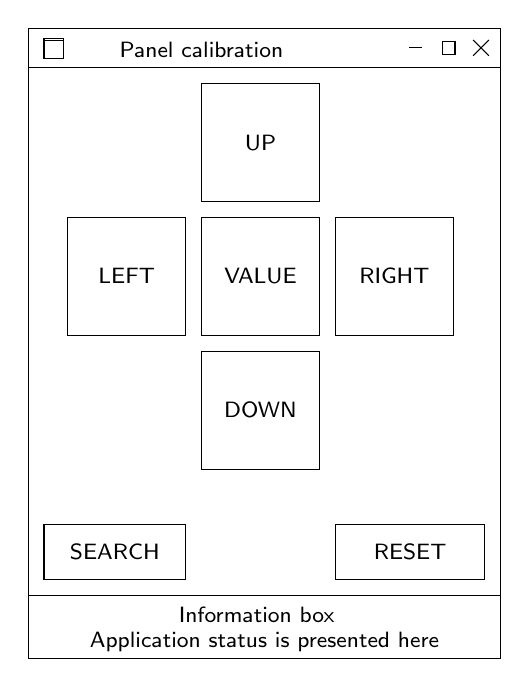
\begin{tikzpicture}[font=\sffamily\footnotesize]
    % Outer rectangle
    \draw (0,0) rectangle (6,8);

    % Top line
    \draw (0,7.5) -- (6,7.5);

    % Bottom line
    \draw (0,0.8) -- (6,0.8);

    % Window functions
    \draw (5.85,7.85) -- (5.65,7.65);           % Close diagonal 1
    \draw (5.85,7.65) -- (5.65,7.85);           % Close diagonal 2
    \draw (5.26,7.67) rectangle (5.42,7.83);    % Maximize (square)
    \draw (4.84,7.75) -- (5.00,7.75);           % Minimize (line)
    \draw (0.2,7.61) rectangle (0.45,7.87);     % Left square
    \draw (0.2,7.84) rectangle (0.45,7.84);     % Line on left square

    % Buttons
    \draw (2.2,7.3) rectangle (3.7,5.8);    % Up
    \draw (0.5,5.6) rectangle (2.0,4.1);    % Left
    \draw (2.2,5.6) rectangle (3.7,4.1);    % Middle
    \draw (3.9,5.6) rectangle (5.4,4.1);    % Right
    \draw (2.2,3.9) rectangle (3.7,2.4);    % Down
    \draw (0.2,1.0) rectangle (2.0,1.7);    % Left corner
    \draw (5.8,1.0) rectangle (3.9,1.7);    % Right corner

    % Text
    \draw (2.2,7.73) node {Panel calibration};
    \draw (2.95,6.55) node {UP};
    \draw (1.25,4.85) node {LEFT};
    \draw (2.95,4.85) node {VALUE};
    \draw (4.65,4.85) node {RIGHT};
    \draw (2.95,3.15) node {DOWN};
    \draw (1.1,1.35) node {SEARCH};
    \draw (4.85,1.35) node {RESET};
    \draw (2.9,0.55) node {Information box};
    \draw (3.0,0.20) node {Application status is presented here};
\end{tikzpicture}
